\documentclass[tikz,border=10pt]{standalone}
\usepackage{tkz-euclide}
\usepackage{tikz}
\usetikzlibrary{calc}

\begin{document}
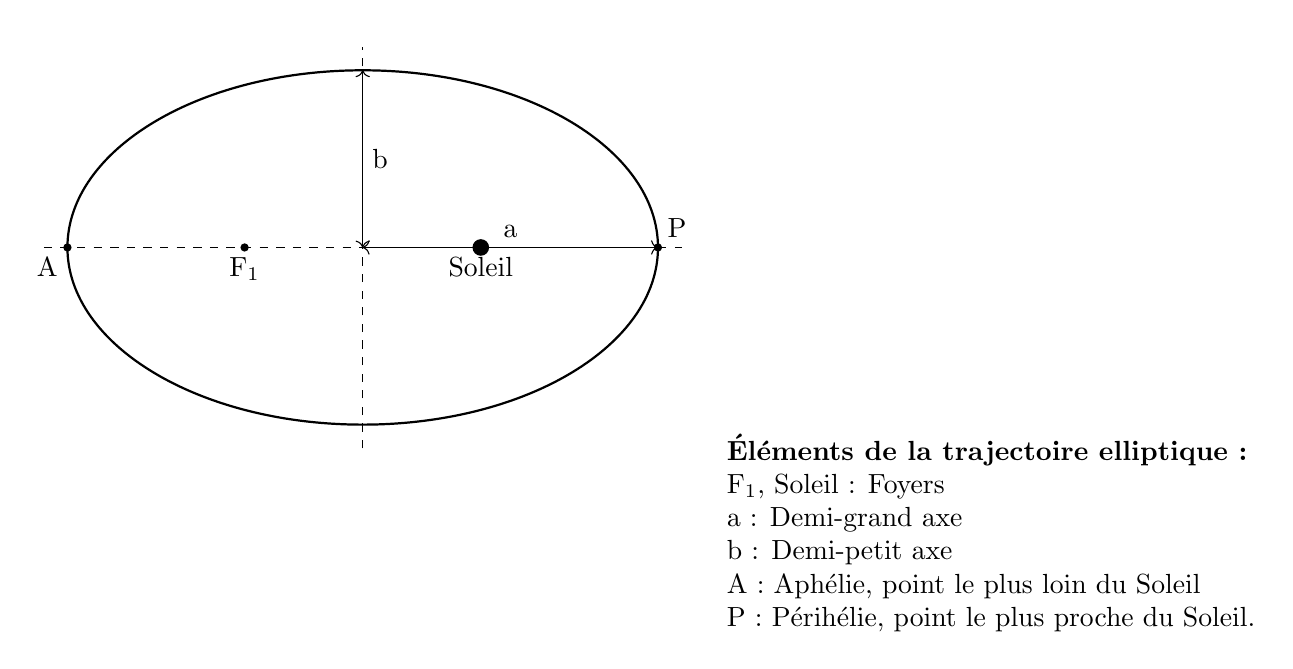
\begin{tikzpicture}[scale=1.5]
    % Définition des points
    \coordinate (C) at (0,0);
    \coordinate (F1) at (-1,0);
    \coordinate (F2) at (1,0);
    \coordinate (A) at (2.5,0);
    \coordinate (B) at (0,1.5);
    % Dessin de l'ellipse
    \draw[thick] (C) ellipse (2.5cm and 1.5cm);

    % Points et labels
    \fill (F1) circle (1pt) node[below] {F$_{1}$};
    \fill (F2) circle (2pt) node[below] {Soleil};
    \fill (A) circle (1pt) node[above right] {P};
    \fill (-2.5,0) circle (1pt) node[ below left] {A};

    % Axes
    \draw[dashed] (-2.7,0) -- (2.7,0) node[right] {};
    \draw[dashed] (0,-1.7) -- (0,1.7) node[above] {};

    % Demi-grand axe et demi-petit axe
    \draw[<->] (C) -- (A) node[midway,above] {a};
    \draw[<->] (C) -- (B) node[midway,right] {b};

    % Distance focale

    % Légende
    \node[align=left, anchor=north west] at (3,-1.5) {
        \textbf{Éléments de la trajectoire elliptique :} \\
        F$_{1}$, Soleil : Foyers \\
        a : Demi-grand axe \\
        b : Demi-petit axe \\
        A : Aphélie, point le plus loin du Soleil\\
        P : Périhélie, point le plus proche du Soleil.};
\end{tikzpicture}
\end{document}
